\documentclass{standalone}
\usepackage{tikz}
\usepackage{amsmath}

\begin{document}

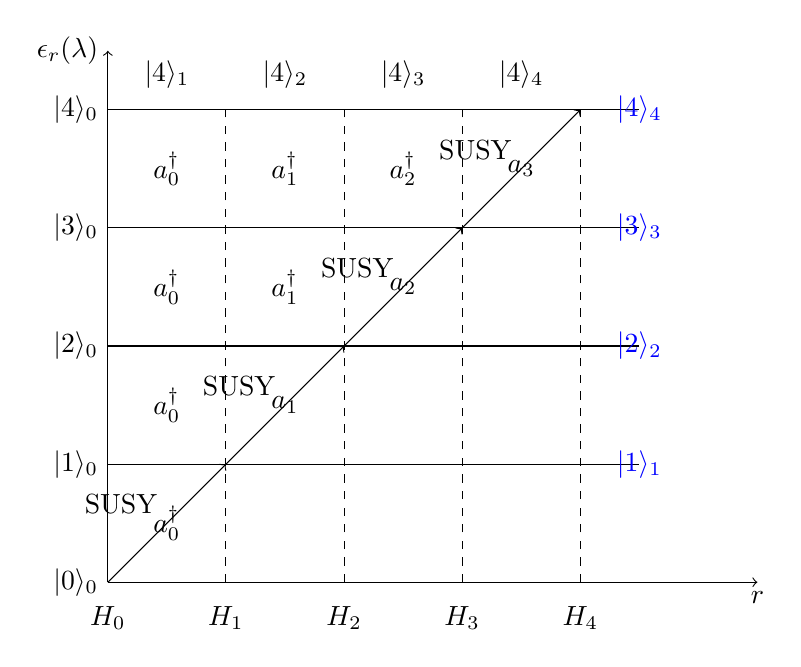
\begin{tikzpicture}[scale=1.5]

% Axes
\draw[->] (0,0) -- (5.5,0) node[anchor=north] {$r$};
\draw[->] (0,0) -- (0,4.5) node[anchor=east] {$\epsilon_r(\lambda)$};

% Hamiltonians
\node at (0,-0.3) {$H_0$};
\node at (1,-0.3) {$H_1$};
\node at (2,-0.3) {$H_2$};
\node at (3,-0.3) {$H_3$};
\node at (4,-0.3) {$H_4$};

% Horizontal lines and labels
\foreach \y in {0,1,2,3,4} {
    \draw (0,\y) -- (4.5,\y);
    \node[anchor=east] at (0,\y) {$|\y\rangle_0$};
}

% Operators a, a^\dagger
\foreach \x/\y/\op in {0/0/a_0^\dagger, 0/1/a_0^\dagger, 0/2/a_0^\dagger, 0/3/a_0^\dagger,
                       1/1/a_1, 1/2/a_1^\dagger, 1/3/a_1^\dagger,
                       2/2/a_2, 2/3/a_2^\dagger,
                       3/3/a_3} {
    \node at (\x+0.5,\y+0.5) {$\op$};
}

% SUSY arrows and labels
\foreach \x/\y/\label in {0/0/SUSY, 1/1/SUSY, 2/2/SUSY, 3/3/SUSY} {
    \draw[->] (\x,\y) -- (\x+1,\y+1);
    \node[anchor=south east] at (\x+0.5,\y+0.5) {\label};
}

% Edge states
\node[blue] at (4.5,4) {$|4\rangle_4$};
\node[blue] at (4.5,3) {$|3\rangle_3$};
\node[blue] at (4.5,2) {$|2\rangle_2$};
\node[blue] at (4.5,1) {$|1\rangle_1$};

% Hamiltonian labels on top
\node at (0.5,4.3) {$|4\rangle_1$};
\node at (1.5,4.3) {$|4\rangle_2$};
\node at (2.5,4.3) {$|4\rangle_3$};
\node at (3.5,4.3) {$|4\rangle_4$};

% Vertical dashed lines
\foreach \x in {1,2,3,4} {
    \draw[dashed] (\x,0) -- (\x,4);
}

\end{tikzpicture}

\end{document}